\section{Materials and Methods}
\label{sec:methodology}

An overview of the proposed method is presented in Fig. \ref{fig:Overview}. Our approach consists of several key components, including depth estimation, adaptive fusion and voting-based grasp generation. These components work synergistically to enhance the dis- criminability and robustness of features, ultimately leading to more accurate and efficient grasp pose generation. We provide a detailed explanation of each of these components and their role in our system’s success.

%%%%%%%%%%%%%%%%%%%%%%%%%%%%%%%%%%%%%%%%%%%%%%%

\begin{figure*}[h!]
	\centering
	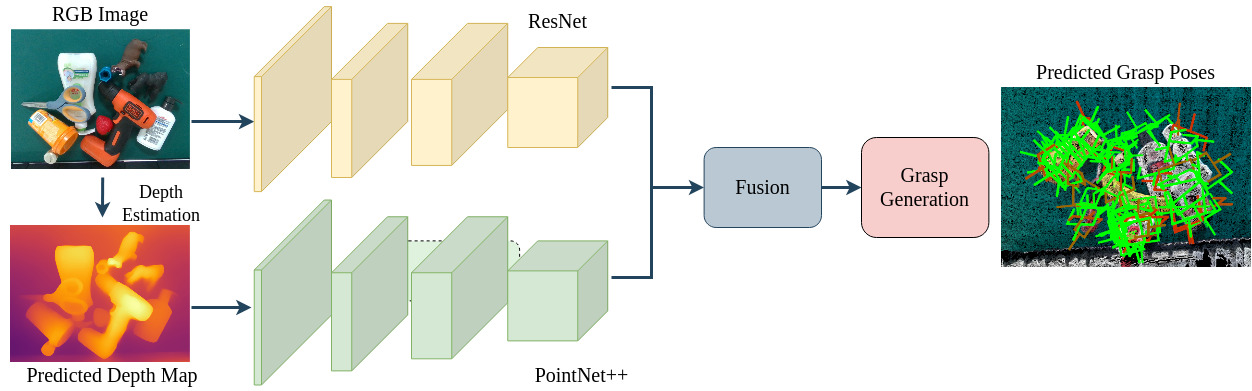
\includegraphics[width=0.98\linewidth]{figs/overview}
	\caption{Overview of our network architecture.}
	\label{fig:Overview}
\end{figure*}
%%%%%%%%%%%%%%%%%%%%%%%%%%%%%%%%%%%%%%%%%%%%%%

\subsection{Depth Estimation}

Given an RGB image $\mathbf{I_v}$, we employ an off-the-shelf monocular depth estimation method to generate a depth map $\mathbf{I}_{d}$. Specifically, we choose DPT \cite{ranftl2021vision}, a dense prediction architecture based on an encoder-decoder design that utilizes a transformer as the fundamental computational building block of the encoder. In particular, DPT adopts the vision transformer (ViT) \cite{dosovitskiy2020image} as its backbone architecture. DPT reconstructs the bag-of-words representation provided by ViT into image-like feature representations at various resolutions. It progressively combines these feature representations into the final dense prediction using a convolutional decoder. Unlike fully-convolutional networks, the vision transformer backbone avoids explicit downsampling operations after computing an initial image embedding and maintains a representation with constant dimensionality throughout all processing stages. Additionally, it ensures a global receptive field at every stage. We demonstrate that these characteristics are particularly advantageous for dense prediction tasks, naturally leading to fine-grained and globally coherent predictions.

\subsection{Feature Extraction and  Fusion}

Given a input RGB image $\mathbf{I_v}$ and an predicted depth map $\mathbf{I_d}$, our initial step involves elevating the depth image $\mathbf{I_d}$ to a point cloud $\mathbf{P}$ using the camera intrinsic matrix. Subsequently, we employ ResNet34 \cite{he2016deep} and PointNet++ \cite{qi2017pointnet++} to extract visual features $\mathcal{F}_{vis}$ from RGB image and geometric feature $\mathcal{F}_{geo}$ from the point cloud $\mathbf{P}$ respectively. 

To achieve the fusion of RGB features $\mathcal{F}_{vis}$ with geometric features $\mathcal{F}_{geo}$, we employ an innovative adaptive fusion module. Departing from the conventional approach of globally compressing the RGB feature map, which may result in the loss of intricate details, we capitalize on the information provided by the aligned RGBD image. The depth information associated with each pixel is instrumental in establishing an XYZ map that is precisely aligned with the RGB map, forming a coherent representation of the scene in three-dimensional space. For each geometric feature, paired with its corresponding 3D point coordinate derived from the aligned RGBD image, we employ a novel strategy to extract pertinent visual information. This involves projecting a defined neighborhood around each 3D point onto the RGB image, utilizing a specified radius $r$. By doing so, we selectively capture the visual context surrounding each point, taking into account its relationship with the RGB features. Subsequently, a crucial step in this fusion process is the extraction of visual features from $\mathcal{F}_{vis}$ for each geometric feature. This is achieved by sampling the $k$ nearest neighbor pixels within the projected neighborhood. The visual features associated with these sampled pixels are then collected and integrated using max pooling. In situations where fewer than $k$ pixels exist in the specified region, null features are padded to maintain the consistency of the sampling process. The collected visual features are then processed through Multi-Layer Perceptrons (MLPs) to ensure their channel size matches that of the original point cloud feature. This modification results in a set of adapted visual features denoted as $\mathcal{F}_{vis}^{'}$, reflecting a refined representation of the RGB information in the context of the geometric features.

Following this adaptation, the integrated visual features $\mathcal{F}_{vis}^{'}$ are concatenated with the original geometric features $\mathcal{F}_{geo}$. This concatenated feature set undergoes further refinement through the application of a shared Multi-Layer Perceptron (MLP), culminating in the generation of the fused geometric feature $\mathcal{F}_{fus}$. This fused representation embodies a synergistic combination of RGB and geometric information, capturing the nuanced interplay between color and spatial features.

Consequently, the network enriches a set of $N$ 3D points with high-dimensional features, denoted as $\mathcal{P} = \lbrace p_i \rbrace_{i=1}^{N}$ and $\mathcal{F}_{fus} = \lbrace f_i \rbrace{i=1}^{N}$, where each $p_i$ is a concatenation of the 3D point's location $x_i \in \mathbb{R}^{3}$ and its associated feature vector $f_i$. The enriched points $\lbrace p_{i} \rbrace_{i=1}^{N}$, now imbued with the fused features, serve as input to our self-attention module, producing enhanced features denoted as $\mathcal{F}$. This self-attention mechanism, inspired by \cite{vaswani2017attention}, dynamically weighs the importance of different enriched features, facilitating the extraction of meaningful relationships and patterns within the spatial context of the 3D points. The resulting enhanced features $\mathcal{F}$ capture the fused information from both RGB and geometric domains, contributing to improved performance in downstream tasks. The self-attention module, as defined in \cite{vaswani2017attention}, is expressed as:

%%%%%%%%%%%%%%%%%%%%%
\begin{equation}
y_{i} = \sum_{p_{j} \in \mathcal{P}(i)} (\alpha(\gamma(p_{i},p_{j}) + \delta) \odot \beta(p_{j}))
\end{equation}
%%%%%%%%%%%%%%%%%%%%%

\noindent Here, $\mathcal{P}(i) \subseteq \mathcal{P}$ refers to a set of points in the local neighborhood of $p_{i}$. The terms $\alpha, \gamma, \delta$, and $\beta$ represent a mapping function, a relation function, a position encoding function, and pointwise feature transformation, respectively. The relation function $\gamma$ utilizes subtraction to output a vector representing the features of $p_i$ and $p_j$:

%%%%%%%%%%%%%%%%%%%%%
\begin{equation}
\gamma(p_{i},p_{j}) = \varphi(p_i) - \psi(p_j)
\end{equation}
%%%%%%%%%%%%%%%%%%%%

\noindent Here, $\varphi$ and $\psi$ are trainable transformations implemented using multilayer perceptrons (MLPs). The mapping function $\alpha$ is an MLP with two linear layers and one ReLU nonlinearity, enabling the module to compute attention weights spatially and across channels while maintaining computational efficiency. To adapt to local data structures, we introduce spatial context using a trainable and parameterized position encoding function $\delta$:

%%%%%%%%%%%%%%%%%%%%%
\begin{equation}
\delta = \phi(x_i - x_j)
\end{equation}
%%%%%%%%%%%%%%%%%%%%

\noindent Here, $x_i$ and $x_j$ denote the 3D point coordinates for points $i$ and $j$, respectively. The encoding function $\phi$ is an MLP with two linear layers and one ReLU nonlinearity. This comprehensive self-attention mechanism allows the network to capture intricate dependencies among enriched features, enhancing the model's capacity for contextualized information processing.

\subsection{Grasp Generation}

Given the extracted dense fused feature $\mathcal{F}=\lbrace{f_i}\rbrace$, we predict grasp poses using the voting-based grasp generation module in our previous work \cite{hoang2023grasp}.

\textbf{Loss Function}: The learning of modules is supervised jointly using a multi-task loss:

\begin{equation}
L_{votegrasp} = \lambda_1 L_{vote} + \lambda_2 L_{grasp}
\label{eq:L_votegrasp_v2}
\end{equation}

The voting loss $L_{vote}$ is a regression loss formulated as:

\begin{equation}
L_{vote} = \frac{1}{M_s} \sum_{i}^{} {\lVert y_i - c^g_i \rVert}_H \cdot \mathds{1}(x_i)
\end{equation}

Here, $M_s$ represents the total number of seed points on the object surface, $c^g_i$ is the closest ground truth grasp center, ${\lVert \cdot \rVert}_H$ denotes the Huber norm, and $\mathds{1}(\cdot)$ is a binary function determining whether a seed point $s_i$ belongs to an object.

The grasp loss function $L_{grasp}$ is defined as:

\begin{equation}
L_{grasp} = L_{center} + \alpha L_{rot} + \beta L_{width} + \gamma L_{score}
\end{equation}

The $L_{grasp}$ comprises losses for grasp center regression ($L_{center}$), rotation ($L_{rot}$), gripper width regression ($L_{width}$), and grasp confidence score regression ($L_{score}$). The grasp center loss includes viewpoint classification loss ($L_{viewpoint}$) and in-plane rotation loss ($L_{in-plane}$), which consists of classification ($L_{angle-cls}$) and regression ($L_{angle-reg}$) losses. Regression losses employ $L1$-smooth loss, while classification losses use standard cross-entropy loss. More details can be found in \cite{hoang2023grasp}.


\subsection{Dataset}

We conduct evaluations and comparisons on the publicly available GraspNet-1Billion dataset \cite{fang2020graspnet}. This dataset comprises 97,280 RGB-D images from 190 cluttered scenes, providing over one billion grasp poses for 88 distinct objects within these scenes. These objects exhibit diversity in shape, texture, size, material, and occlusion conditions, making it an ideal benchmark for assessing our model's generalization capacity and robustness to occlusions. Each object in the dataset is associated with an accurate 3D mesh model, along with camera poses, 6D object poses, object masks, and bounding boxes for all frames. This extensive annotation facilitates straightforward generation of ground truth votes and grasp configurations. Following the methodology of \cite{fang2020graspnet}, we partitioned the dataset into training and testing sets. Specifically, 100 scenes were allocated for training purposes, while 90 scenes were reserved for testing. To evaluate the model's generalizability, the test dataset is further divided into subsets: scenes with novel objects, scenes featuring unseen yet similar objects, and scenes containing previously encountered objects. This deliberate partitioning allows for a comprehensive assessment of our model's performance across diverse scenarios.
